% Author: Mark Weinreuter		
\newcommand*{\VorlagenPfad}{../../../../Vorlagen}
\documentclass{\VorlagenPfad/coderdojokatext}

\newcommand{\Titel}{Variablen}

\begin{document}


\begin{center}
	{\huge \Titel}
\end{center}

\section{Was sind Variablen}
Als Programmier sind Variablen deine besten Freunde. Variablen werden benutzt, um darin Werte zu speichern. Du kannst sie dir wie eine kleine Schublade vorstellen. Auf der Schublade steht der Name deiner Variablen. Du kannst die Schublade aufmachen und einen Wert z.B. eine Zahl reinlegen. Genauso kannst du zu jeder Zeit die Schublade aufmachen, um den Wert zu lesen.

\begin{center}
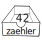
\includegraphics[width=6cm]{schublade}
\end{center}

\subsection{Variablen in Python}
In Python sieht das Ganze so aus:

\inputminted[firstline=1, lastline=4]{python}{../../../Beispiele/variablen.py}

Auf der linken Seite steht der Name der Variablen, die erstellt wird. Auf der rechten Seite steht der Wert, der ihr zugewiesen wird.
Mithilfe des \code{print}-Befehls, kann der Wert einer Variablen ausgegeben werden.


\inputminted[firstline=7, lastline=8]{python}{../../../Beispiele/variablen.py}
Der Wert der Variablen kann ganz leicht geändert werden.

\subsection{Rechnen mit Variablen}
Man kann Zahlen in Variablen speichern, warum also nicht auch mit ihnen rechnen.
\inputminted[firstline=11, lastline=15]{python}{../../../Beispiele/variablen.py}

Hier gibt es zwei neue Variablen, \code{zahl} und \code{ergebnis}. Die Variable \code{ergebnis} wird mit dem Wert
von \code{zahl} multipliziert mit 5 initialisiert.

\inputminted[firstline=16, lastline=21]{python}{../../../Beispiele/variablen.py}
Es können alle Grundoperationen wie Plus, Minus, Mal, Geteilt verwendet werden. Allerdings sind hierbei Rechenregeln wie 'Punkt vor Strich' zu beachten.

\subsection{Merkregel}
\begin{merkbox}
	Um eine Variable zu erzeugen/verändern steht die Variable auf der linken Seite des '='-Zeichens.
\begin{pythoncode}
zahl = ...
\end{pythoncode}
Um den Wert zu lesen steht die Variable auf der rechten Seite des '='-Zeichens.
\begin{pythoncode}
... = zahl + 1
\end{pythoncode}

\end{merkbox}

\subsection{Variablen mit sich selbst verrechnen}
Am Anfang mag es vielleicht etwas verwirrend erscheinen, aber man kann den Wert einer Variablen überschreiben, indem man den vorherigen Wert in einer Berechnung verwendet:

\inputminted[firstline=23, lastline=26]{python}{../../../Beispiele/variablen.py}
Hier gilt einfach die Merkregel von oben. Zuerst wird die rechte Seite berechnet. Es wird der Wert von \code{zahl} gelsen und \code{1} dazu addiert. Dann wird der Wert von \code{zahl} mit dem neuen Wert überschrieben.

\section{Aufgaben}
Damit du mit Variablen vertrauter wirst, spiele einfach ein bisschen damit rum.
\begin{itemize}
	\item Erstelle eine Variable und ändere mehrmals ihren Wert
	\item Gib den Wert deiner Variablen mit \code{print} aus und sie wie er sich verändert
	\item Überschreibe den Wert deiner Variablen mit 10-fachen des ursprünglichen Wertes
	\item Finde heraus, welche Buchstaben, Zahlen, Sonderzeichen in Variablen erlaubt sind. Um dies auszuprobieren starte mit einem Namen der nur Bustaben enthält, z.B. \code{zahl}. Starte das Programm, es sollte erfolgreich durchlaufen. Füge nun neue Zeichen hinzu und teste erneut das Program. 
\end{itemize}

\section{Ausblick}
Man kann in Variablen natürlich nicht nur Zahlen speichern. Es kann z.B. auch Text darin gespeichert werden.
\inputminted[firstline=28, lastline=31]{python}{../../../Beispiele/variablen.py}
Mehr Infos zum Umgang mit Text findest du in dem Tutorial dazu

\end{document}